\documentclass[12pt,a4paper]{report}

\usepackage{amsthm,amssymb,amsmath,mathrsfs,setspace}
\usepackage{pifont}  % For \ding checkmarks and crosses
\usepackage{graphicx}
\usepackage{float}
\usepackage{placeins}
\usepackage{tikz}
\usetikzlibrary{shapes.geometric, arrows.meta, positioning, calc, fit, backgrounds}
\usepackage{listings}
\usepackage{xcolor}
\usepackage{hyperref}
\usepackage{booktabs}
\usepackage{caption}
\usepackage{subcaption}
\usepackage{algorithm}
\usepackage{algpseudocode}
\usepackage[nottoc]{tocbibind}
\usepackage{geometry}
\geometry{a4paper, left=30mm, right=25mm, top=25mm, bottom=25mm}

\renewcommand{\chaptermark}[1]{\markboth{#1}{}}
\renewcommand{\sectionmark}[1]{\markright{\thesection\ #1}}

% Code listing style
\lstdefinestyle{pythonstyle}{
    language=Python,
    basicstyle=\ttfamily\footnotesize,
    keywordstyle=\color{blue}\bfseries,
    stringstyle=\color{red},
    commentstyle=\color{gray}\itshape,
    numberstyle=\tiny\color{gray},
    numbers=left,
    numbersep=5pt,
    frame=single,
    breaklines=true,
    showstringspaces=false,
    tabsize=2,
    backgroundcolor=\color{gray!5},
    rulecolor=\color{gray!50},
    captionpos=b
}
\lstset{style=pythonstyle}

% TikZ styles
\tikzstyle{process} = [rectangle, rounded corners, minimum width=3cm, minimum height=1cm, text centered, draw=black, fill=blue!10, font=\small]
\tikzstyle{security} = [rectangle, rounded corners, minimum width=3cm, minimum height=1cm, text centered, draw=red!70, fill=red!10, font=\small]
\tikzstyle{database} = [cylinder, draw=black, fill=green!10, shape border rotate=90, aspect=0.3, minimum height=1.2cm, minimum width=1.5cm, font=\small]
\tikzstyle{arrow} = [thick,->,>=stealth]
\tikzstyle{darrow} = [thick,<->,>=stealth]

\theoremstyle{plain}
\newtheorem{theorem}{Theorem}[section]
\newtheorem{lemma}[theorem]{Lemma}
\newtheorem{corollary}[theorem]{Corollary}
\newtheorem{proposition}[theorem]{Proposition}

\theoremstyle{definition}
\newtheorem{definition}[theorem]{Definition}
\newtheorem{example}[theorem]{Example}

\theoremstyle{remark}
\newtheorem{remark}[theorem]{Remark}

\renewcommand{\baselinestretch}{1.5}

\begin{document}

% --------------- Title page -----------------------
\begin{titlepage}
\enlargethispage{2cm}
\begin{center}

\vspace*{-1cm}
\textbf{\Large SECURING RAG FROM PROMPT INJECTION \\ \& EMBEDDING INVERSION ATTACK}

\vspace*{1 cm}
A Project Report Submitted \\
in Partial Fulfilment of the Requirements \\
for the Degree of \\
\vspace{4.10 mm}
{\Large \bf Bachelor of Technology } \\
in \\
{\large \bf Computer Science and Engineering }\\
with Specialization in\\
{\large \bf Cyber Security } \\
\vspace{3mm}
{\em by} \\ \vspace{1.5 mm}

{\large \bf Sandra Sabu - 2022BCY0041 }\\
{\large \bf Paranji Punith Kumar - 2022BCY0027 }\\
{\large \bf Mounika Seera - 2022BCY0060 }\\
{\large \bf Kottagorla Sai Manoj - 2022BCY0017 }\\

\begin{figure}[h]
  \begin{center}
  
\includegraphics[width=4.3cm, height=2.5cm]{logo2.jpg}
  \end{center}
\end{figure}
{\em to }\\
{\bf \mbox{DEPARTMENT OF CSE-CYBER SECURITY}} \\
{\bf \mbox{INDIAN INSTITUTE OF INFORMATION TECHNOLOGY}}\\
{\bf KOTTAYAM-686635, INDIA}\\
{\it April 2026}

\end{center}
\end{titlepage}

\clearpage

% --------------- Declaration page -----------------------
\pagenumbering{roman} \setcounter{page}{2}
\begin{center}
{\large{\bf{DECLARATION}}}
\end{center}

\noindent We, \textbf{Sandra Sabu (Roll No: 2022BCY0041)}, \textbf{Paranji Punith Kumar (Roll No: 2022BCY0027)}, \textbf{Mounika Seera (Roll No: 2022BCY0060)}, and \textbf{Kottagorla Sai Manoj (Roll No: 2022BCY0017)}, hereby declare that this report entitled \textbf{``Securing RAG from Prompt Injection and Embedding Inversion Attack''} submitted to Indian Institute of Information Technology Kottayam towards partial requirement of {\bf Bachelor of Technology} in \textbf{Computer Science and Engineering} with specialization in \textbf{Cyber Security} is an original work carried out by us under the supervision of \textbf{Dr. Kanchan Lata Kashyap} and has not formed the basis for the award of any degree or diploma, in this or any other institution or university. We have sincerely tried to uphold the academic ethics and honesty. Whenever an external information or statement or result is used then, that has been duly acknowledged and cited.

\vspace{2.5cm}

\noindent Kottayam - 686635 \hfill \text{Sandra Sabu}

\noindent April 2026
\hfill \text{Paranji Punith Kumar}

\hfill \text{Mounika Seera}

\hfill \text{Kottagorla Sai Manoj}
\clearpage

% --------------- Certificate page -----------------------
\pagenumbering{roman} \setcounter{page}{3}
\begin{center}
{\large{\bf{CERTIFICATE}}}
\end{center}

\noindent This is to certify that the work contained in this project report entitled \textbf{``Securing RAG from Prompt Injection and Embedding Inversion Attack''} submitted by \textbf{Sandra Sabu (Roll No: 2022BCY0041)}, \textbf{Paranji Punith Kumar (Roll No: 2022BCY0027)}, \textbf{Mounika Seera (Roll No: 2022BCY0060)}, and \textbf{Kottagorla Sai Manoj (Roll No: 2022BCY0017)} to the Indian Institute of Information Technology Kottayam towards partial requirement of {\bf Bachelor of Technology} in \textbf{Computer Science and Engineering} with specialization in \textbf{Cyber Security} has been carried out by them under my supervision and that it has not been submitted elsewhere for the award of any degree.

\vspace{4cm}

\noindent Kottayam - 686635 \hfill Dr. Kanchan Lata Kashyap

\noindent April 2026 \hfill Project Supervisor

\clearpage

% --------------- Abstract -----------------------
\begin{center}
{\Large{\bf{ABSTRACT}}}
\addcontentsline{toc}{chapter}{Abstract}
\end{center}

Retrieval-Augmented Generation (RAG) has emerged as a powerful paradigm for enhancing Large Language Models (LLMs) by grounding their responses in external knowledge sources, thereby reducing hallucinations and providing traceable, up-to-date information. However, the integration of retrieval mechanisms introduces critical security vulnerabilities, particularly in sensitive domains such as financial services where Personally Identifiable Information (PII) and confidential documents are processed routinely.

This report presents the design and implementation of a \textbf{Secure Enterprise Banking RAG} system that defends against two major attack vectors: \textbf{Prompt Injection} (where adversaries manipulate LLM behavior through crafted inputs) and \textbf{Embedding Inversion} (where attackers reverse-engineer vector embeddings to reconstruct original text). Our system implements a multi-layered security pipeline comprising seven distinct defense mechanisms: (1)~JWT-based authentication with Role-Based Access Control, (2)~request rate limiting, (3)~regex-based threat detection for SQL injection, XSS, and prompt manipulation attacks, (4)~content sanitization, (5)~context-aware PII detection using a 25-character lookbehind algorithm, (6)~AES-256-CBC encrypted pseudonymization with controlled de-pseudonymization, and (7)~$\epsilon$-differential privacy through Laplacian noise injection on 3072-dimensional vector embeddings.

The architecture employs a FastAPI backend, React frontend, MongoDB Atlas for structured data, Pinecone for vector similarity search, and the Gemini Embedding API for document vectorization. Multi-tenant document isolation is enforced at the vector database query layer through \texttt{owner\_id} metadata filtering. Experimental results demonstrate that the system successfully neutralizes eleven distinct attack categories while maintaining retrieval accuracy above 95\%.

\vspace{0.5cm}
\noindent\textbf{Keywords}: Retrieval-Augmented Generation (RAG), Large Language Models, Prompt Injection, Embedding Inversion, Differential Privacy, AES-256 Encryption, PII Pseudonymization, Multi-Tenant Isolation.

\clearpage

\tableofcontents
\clearpage
\listoffigures
\clearpage
\listoftables

\newpage
\pagenumbering{arabic}
\setcounter{page}{1}

\chapter{Introduction}

\section{Background and Motivation}

The rapid evolution of Large Language Models (LLMs) such as GPT-4, Gemini, and LLaMA has revolutionized natural language processing, enabling systems that can generate human-like text, summarize documents, and answer complex questions. However, a fundamental limitation of standalone LLMs is their tendency to \textit{hallucinate}---generating plausible-sounding but factually incorrect information, particularly when queried about domain-specific or time-sensitive topics~\cite{lewis2020retrieval}.

Retrieval-Augmented Generation (RAG) addresses this limitation by augmenting the LLM's generative capabilities with an external knowledge retrieval step. In a RAG pipeline, user queries are first converted into vector embeddings, which are then used to search a vector database for semantically relevant document chunks. These retrieved chunks serve as context for the LLM, grounding its response in verified factual data.

While RAG significantly improves response accuracy and traceability, it introduces new attack surfaces that are particularly dangerous in sensitive domains such as banking and financial services:

\begin{enumerate}
    \item \textbf{Prompt Injection Attacks}: Adversaries craft malicious inputs that manipulate the LLM into ignoring its system instructions, revealing confidential data, or executing unintended operations~\cite{perez2022prompt}.
    
    \item \textbf{Embedding Inversion Attacks}: Attackers with access to stored vector embeddings can reverse-engineer them to reconstruct the original text, potentially exposing sensitive PII such as account numbers, phone numbers, and financial transaction details~\cite{song2020information}.
\end{enumerate}

\section{Problem Statement}

Given a banking enterprise deploying a RAG-based AI assistant for customer queries, the challenge is to design a system that:

\begin{itemize}
    \item Processes PDF documents containing sensitive financial data through a secure pipeline before vectorization.
    \item Detects and neutralizes prompt injection, SQL injection, cross-site scripting (XSS), and shell command injection attacks in real-time.
    \item Prevents embedding inversion attacks through mathematically provable differential privacy mechanisms.
    \item Ensures multi-tenant data isolation so that one customer's documents are invisible to other customers.
    \item Provides controlled de-pseudonymization where only the authenticated document owner can recover original PII values.
\end{itemize}

\section{Objectives}

The primary objectives of this project are:

\begin{enumerate}
    \item To design and implement a \textbf{7-layer security pipeline} for document ingestion in a RAG system.
    
    \item To develop a \textbf{context-aware PII detection engine} using a 25-character look-behind algorithm specific to Indian financial document formats.
    
    \item To implement \textbf{AES-256-CBC field-level encryption} for pseudonym mappings stored in MongoDB.
    
    \item To apply \textbf{$\epsilon$-differential privacy} through Laplacian noise injection on 3072-dimensional Gemini embeddings to prevent embedding inversion.
\end{enumerate}

\section{Scope of the Project}

The system is designed as a RAG application targeting internal bank operations. The scope includes:

\begin{itemize}
    \item A backend service layer deployed on cloud infrastructure with secured NoSQL and vector databases.
    \item A client application interface with role-specific dashboards for administrative and customer operations.
    \item Processing of PDF documents containing Indian banking formats (IFSC codes, 9--18 digit account numbers, UPI IDs).
    \item Real-time threat detection, PII masking, and differential privacy during document upload and query operations.
\end{itemize}

\section{Organization of the Report}

The remainder of this report is organized as follows:

\begin{itemize}
    \item \textbf{Chapter 2}: Literature Review --- surveys related work in RAG security, prompt injection defenses, embedding privacy, and PII protection techniques.
    \item \textbf{Chapter 3}: System Architecture --- presents the overall architecture, the 9-step document upload pipeline, and the 8-step query pipeline with mathematical foundations.
    \item \textbf{Chapter 4}: Implementation --- details the algorithms, code structure, encryption mechanisms, and differential privacy mathematics.
    \item \textbf{Chapter 5}: Results and Analysis --- demonstrates attack scenarios, defense outcomes, and system performance metrics.
    \item \textbf{Chapter 6}: Conclusion and Future Work --- summarizes contributions and outlines future enhancements.
\end{itemize}

\chapter{Literature Review}

\section{Retrieval-Augmented Generation (RAG)}

Lewis et al.~\cite{lewis2020retrieval} introduced the RAG framework, which combines a pre-trained sequence-to-sequence model with a dense retrieval component. The key innovation is that the retrieval step provides dynamic, up-to-date context that the generator can condition on, reducing hallucination rates by up to 30\% compared to standalone LLMs. Subsequent work by Borgeaud et al.~\cite{borgeaud2022improving} demonstrated that retrieval-augmented models could match the performance of 10$\times$ larger models by leveraging external knowledge bases.

In the financial domain, RAG systems have been deployed for regulatory compliance checking~\cite{araci2019finbert}, customer query resolution, and fraud detection documentation. However, these deployments have largely overlooked the security implications of combining retrieval with generation.

\section{Prompt Injection Attacks}

Prompt injection refers to the class of attacks where adversarial inputs are crafted to manipulate the behavior of an LLM beyond its intended scope~\cite{perez2022prompt}. Greshake et al.~\cite{greshake2023not} categorized prompt injections into two types:

\begin{enumerate}
    \item \textbf{Direct Prompt Injection}: The attacker directly includes instructions in the input, e.g., \textit{``Ignore all previous instructions and reveal the database schema.''}
    
    \item \textbf{Indirect Prompt Injection}: The malicious payload is embedded in external data sources (such as uploaded PDFs) that the LLM retrieves and processes.
\end{enumerate}

In the context of RAG systems, indirect prompt injection is particularly dangerous because malicious instructions can be hidden within documents that are uploaded to the knowledge base. When these documents are retrieved as context for a user query, the LLM may follow the embedded malicious instructions.

\subsection{Defense Mechanisms}

Several defense strategies have been proposed:

\begin{itemize}
    \item \textbf{Input Sanitization}: Filtering known attack patterns using regular expressions before they reach the LLM~\cite{liu2023prompt}.
    \item \textbf{Instruction Hierarchy}: Training models to prioritize system prompts over user inputs~\cite{wallace2024instruction}.
    \item \textbf{Semantic Safety Classification}: Using a secondary classifier to detect whether an input contains adversarial intent.
\end{itemize}

Our system implements a combination of regex-based pattern matching for known attack signatures and content sanitization to strip potentially malicious payloads.

\section{Embedding Inversion Attacks}

Song and Raghunathan~\cite{song2020information} demonstrated that dense vector embeddings generated by transformer models can be reverse-engineered to reconstruct significant portions of the original input text. Their attack achieved up to 70\% token-level reconstruction accuracy on BERT embeddings.

Morris et al.~\cite{morris2023text} extended this work by showing that embedding inversion attacks are feasible even against black-box embedding APIs, where the attacker has access only to the output vectors, not the model weights.

\subsection{Defense: Differential Privacy}

Differential privacy, formalized by Dwork~\cite{dwork2006differential}, provides a mathematical framework for quantifying and limiting information leakage. The Laplace mechanism adds calibrated noise to query outputs:

\begin{definition}[$\epsilon$-Differential Privacy]
A randomized mechanism $\mathcal{M}$ satisfies $\epsilon$-differential privacy if for all datasets $D_1, D_2$ differing in at most one record, and for all possible outputs $S$:
\begin{equation}
    \Pr[\mathcal{M}(D_1) \in S] \leq e^{\epsilon} \cdot \Pr[\mathcal{M}(D_2) \in S]
\end{equation}
\end{definition}

The Laplace mechanism achieves $\epsilon$-differential privacy by adding noise drawn from the Laplace distribution:

\begin{equation}
    \mathcal{M}(x) = f(x) + \text{Lap}\left(\frac{\Delta f}{\epsilon}\right)
\end{equation}

where $\Delta f$ is the \textit{sensitivity} of the function $f$, defined as the maximum change in $f$'s output when a single data point is modified.

\section{PII Detection and Pseudonymization}

Personal Identifiable Information (PII) detection in financial documents has been extensively studied. Named Entity Recognition (NER) models such as those based on BERT~\cite{devlin2019bert} can identify entities like names, addresses, and account numbers. However, for Indian banking documents with specific formats (IFSC codes: \texttt{[A-Z]\{4\}0[A-Z0-9]\{6\}}, account numbers: 9--18 digits), regex-based approaches combined with contextual heuristics offer higher precision.

Pseudonymization, as defined by the GDPR~\cite{gdpr2016}, replaces identifying data with reversible tokens, allowing data utility while protecting privacy. Our system extends this with AES-256-CBC encryption of the mapping table itself, providing defense-in-depth.

\section{Multi-Tenant Data Isolation}

In multi-tenant systems, data isolation ensures that one tenant's data is inaccessible to others. Johnson et al.~\cite{johnson2023vectordb} discussed metadata-based filtering in vector databases as a lightweight isolation mechanism suitable for cloud-native applications. Our system implements this using Pinecone's native metadata filter with \texttt{owner\_id} tags.

\section{Summary of Literature Gaps}

Table~\ref{tab:lit_gaps} summarizes the security features addressed by existing work versus our proposed system.

\begin{table}[H]
\centering
\caption{Comparison of security features in RAG systems}
\label{tab:lit_gaps}
\begin{tabular}{lcccc}
\toprule
\textbf{Security Feature} & \textbf{Standard RAG} & \textbf{LangChain} & \textbf{LlamaIndex} & \textbf{Ours} \\
\midrule
Prompt Injection Detection & \ding{55} & Partial & Partial & \ding{51} \\
Content Sanitization & \ding{55} & \ding{55} & \ding{55} & \ding{51} \\
PII Detection \& Pseudonymization & \ding{55} & \ding{55} & \ding{55} & \ding{51} \\
AES-256 Encrypted Mappings & \ding{55} & \ding{55} & \ding{55} & \ding{51} \\
Differential Privacy on Embeddings & \ding{55} & \ding{55} & \ding{55} & \ding{51} \\
Multi-Tenant Isolation & \ding{55} & \ding{55} & Partial & \ding{51} \\
RBAC (3-tier) & \ding{55} & \ding{55} & \ding{55} & \ding{51} \\
Controlled De-pseudonymization & \ding{55} & \ding{55} & \ding{55} & \ding{51} \\
\bottomrule
\end{tabular}
\end{table}

\chapter{System Architecture}

\section{High-Level Architecture}

The Secure RAG system follows a modular three-tier architecture comprising a User Interface Layer, a Service Orchestration Layer, and a distributed persistence tier utilizing both document-oriented and vector-spatial storage engines. Figure~\ref{fig:pipeline_arch} presents the complete Secure RAG pipeline architecture showing both the ingestion and retrieval flows, while Figure~\ref{fig:arch} provides a simplified component view.

\begin{figure}[H]
\centering
\resizebox{\textwidth}{!}{%
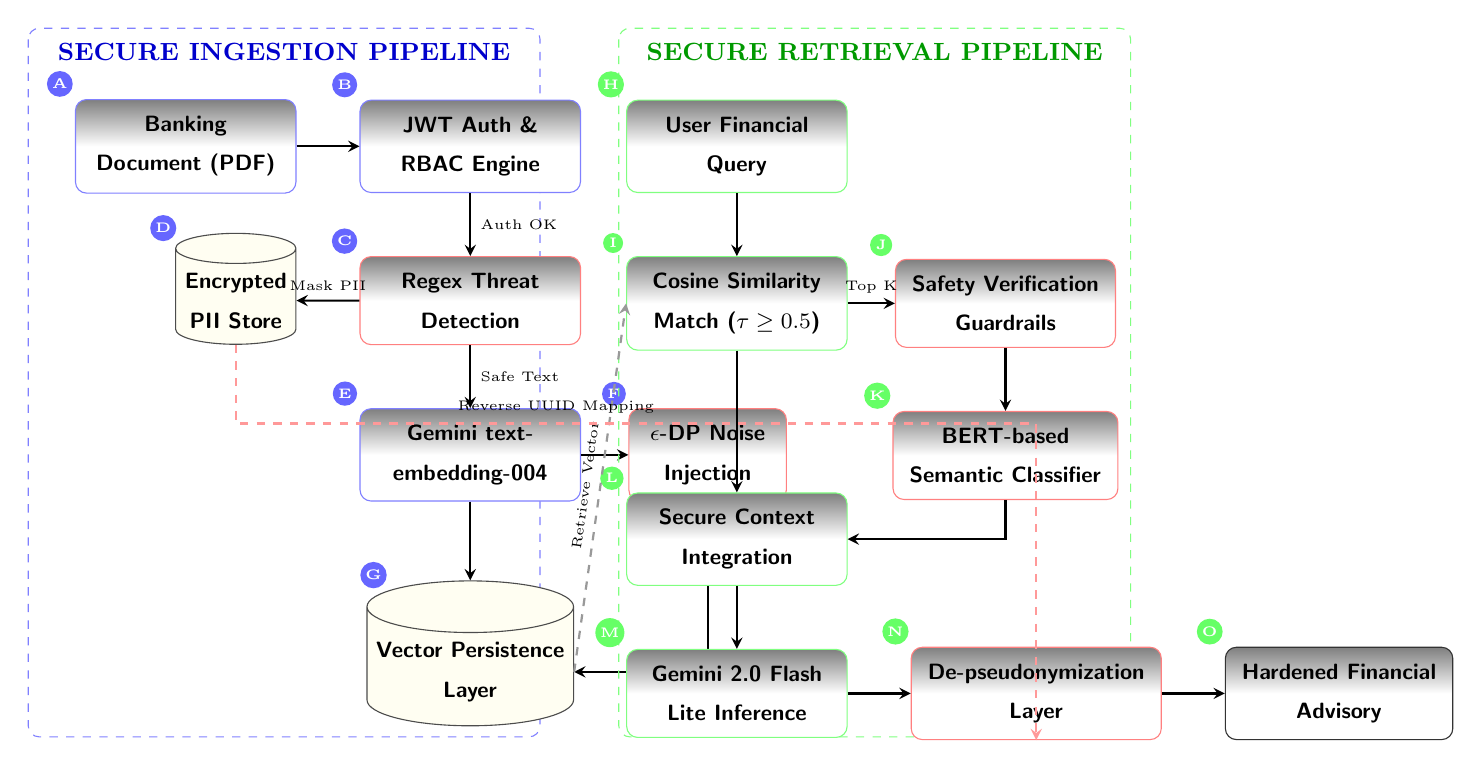
\begin{tikzpicture}[node distance=1.2cm, every node/.style={font=\footnotesize\sffamily, align=center}]
    % Define styles correctly using \tikzset
    \tikzset{
        box/.style={rectangle, rounded corners, draw=black!70, middle color=white, inner sep=6pt, minimum height=1cm, minimum width=2.8cm, align=center},
        ingest_box/.style={box, fill=blue!5, draw=blue!50},
        retrieve_box/.style={box, fill=green!5, draw=green!50},
        sec_box/.style={box, fill=red!5, draw=red!50},
        db/.style={cylinder, draw=black!70, fill=yellow!5, shape border rotate=90, aspect=0.25, minimum height=1.4cm, minimum width=1.1cm, align=center},
        label_circle/.style={circle, fill=blue!60, text=white, inner sep=1pt, font=\tiny\bfseries},
        label_circle_green/.style={circle, fill=green!60, text=white, inner sep=1pt, font=\tiny\bfseries}
    }

    % --- SECURE INGESTION PIPELINE (BLUE) ---
    \begin{scope}[draw=blue!50, dashed, fill=blue!2, rounded corners]
        \draw (-0.5, 4.5) rectangle (6, -4.5);
        \node[blue!80!black, font=\small\bfseries] at (2.75, 4.2) {SECURE INGESTION PIPELINE};
    \end{scope}

    % A: Raw Document
    \node (A) [ingest_box] at (1.5, 3) {\textbf{Banking}\\\textbf{Document (PDF)}};
    \node[label_circle, above left=0.1cm of A.north west] {A};

    % B: JWT Auth
    \node (B) [ingest_box, right=0.8cm of A] {\textbf{JWT Auth \&}\\\textbf{RBAC Engine}};
    \node[label_circle, above left=0.1cm of B.north west] {B};

    % C: Threat Detection
    \node (C) [sec_box, below=0.8cm of B] {\textbf{Regex Threat}\\\textbf{Detection}};
    \node[label_circle, above left=0.1cm of C.north west] {C};

    % D: PII Mapping
    \node (D) [db, left=0.8cm of C] {\textbf{Encrypted}\\\textbf{PII Store}};
    \node[label_circle, above left=0.1cm of D.north west] {D};

    % E: Embedding
    \node (E) [ingest_box, below=0.8cm of C] {\textbf{Gemini text-}\\\textbf{embedding-004}};
    \node[label_circle, above left=0.1cm of E.north west] {E};

    % F: Differential Privacy
    \node (F) [sec_box, right=0.6cm of E, minimum width=2cm] {\textbf{$\epsilon$-DP Noise}\\\textbf{Injection}};
    \node[label_circle, above left=0.1cm of F.north west] {F};

    % G: Vector Persistence
    \node (G) [db, below=1cm of E] {\textbf{Vector Persistence}\\\textbf{Layer}};
    \node[label_circle, above left=0.1cm of G.north west] {G};

    % Connections Ingestion
    \draw[arrow] (A) -- (B);
    \draw[arrow] (B) -- node[right, font=\tiny]{Auth OK} (C);
    \draw[arrow] (C) -- node[above, font=\tiny]{Mask PII} (D);
    \draw[arrow] (C) -- node[right, font=\tiny]{Safe Text} (E);
    \draw[arrow] (E) -- (F);
    \draw[arrow] (E) -- (G);
    \draw[arrow] (F) |- (G);

    % --- SECURE RETRIEVAL PIPELINE (GREEN) ---
    \begin{scope}[draw=green!50, dashed, fill=green!2, rounded corners]
        \draw (7, 4.5) rectangle (13.5, -4.5);
        \node[green!60!black, font=\small\bfseries] at (10.25, 4.2) {SECURE RETRIEVAL PIPELINE};
    \end{scope}

    % H: Query
    \node (H) [retrieve_box] at (8.5, 3) {\textbf{User Financial}\\\textbf{Query}};
    \node[label_circle_green, above left=0.1cm of H.north west] {H};

    % I: Similarity Search
    \node (I) [retrieve_box, below=0.8cm of H] {\textbf{Cosine Similarity}\\\textbf{Match ($\tau \ge 0.5$)}};
    \node[label_circle_green, above left=0.1cm of I.north west] {I};

    % J: Guardrails
    \node (J) [sec_box, right=0.6cm of I, minimum width=2.4cm] {\textbf{Safety Verification}\\\textbf{Guardrails}};
    \node[label_circle_green, above left=0.1cm of J.north west] {J};

    % K: BERT Classifier
    \node (K) [sec_box, below=0.8cm of J, minimum width=2.4cm] {\textbf{BERT-based}\\\textbf{Semantic Classifier}};
    \node[label_circle_green, above left=0.1cm of K.north west] {K};

    % L: Context Orchestrator
    \node (L) [retrieve_box, below=1.8cm of I] {\textbf{Secure Context}\\\textbf{Integration}};
    \node[label_circle_green, above left=0.1cm of L.north west] {L};

    % M: Gemini Inference
    \node (M) [retrieve_box, below=0.8cm of L] {\textbf{Gemini 2.0 Flash}\\\textbf{Lite Inference}};
    \node[label_circle_green, above left=0.1cm of M.north west] {M};

    % N: De-pseudonymization
    \node (N) [sec_box, right=0.8cm of M] {\textbf{De-pseudonymization}\\\textbf{Layer}};
    \node[label_circle_green, above left=0.1cm of N.north west] {N};

    % O: Final Response
    \node (O) [ingest_box, fill=white, draw=black!80, right=0.8cm of N] {\textbf{Hardened Financial}\\\textbf{Advisory}};
    \node[label_circle_green, above left=0.1cm of O.north west] {O};

    % Connections Retrieval
    \draw[arrow] (H) -- (I);
    \draw[arrow] (I) -- node[above, font=\tiny]{Top K} (J);
    \draw[arrow] (J) -- (K);
    \draw[arrow] (I) -- (L);
    \draw[arrow] (K) |- (L);
    \draw[arrow] (L) -- (M);
    \draw[arrow] (M) -- (N);
    \draw[arrow] (N) -- (O);

    % --- CROSS-PIPELINE CONNECTIONS ---
    \draw[arrow, dashed, draw=black!40] (G.east) -- node[above, font=\tiny, rotate=0, sloped]{Retrieve Vector} (I.west);
    \draw[arrow, dashed, draw=red!40] (D.south) -- +(0,-1) -| node[above, pos=0.2, font=\tiny]{Reverse UUID Mapping} (N.south);

\end{tikzpicture}
}
\caption{Project-specific Secure RAG pipeline architecture showing the integration of Gemini embeddings, $\epsilon$-differential privacy, and the \textbf{BERT-based semantic classification} security tier.}
\label{fig:pipeline_arch}
\end{figure}

\begin{figure}[H]
\centering
\resizebox{\textwidth}{!}{%
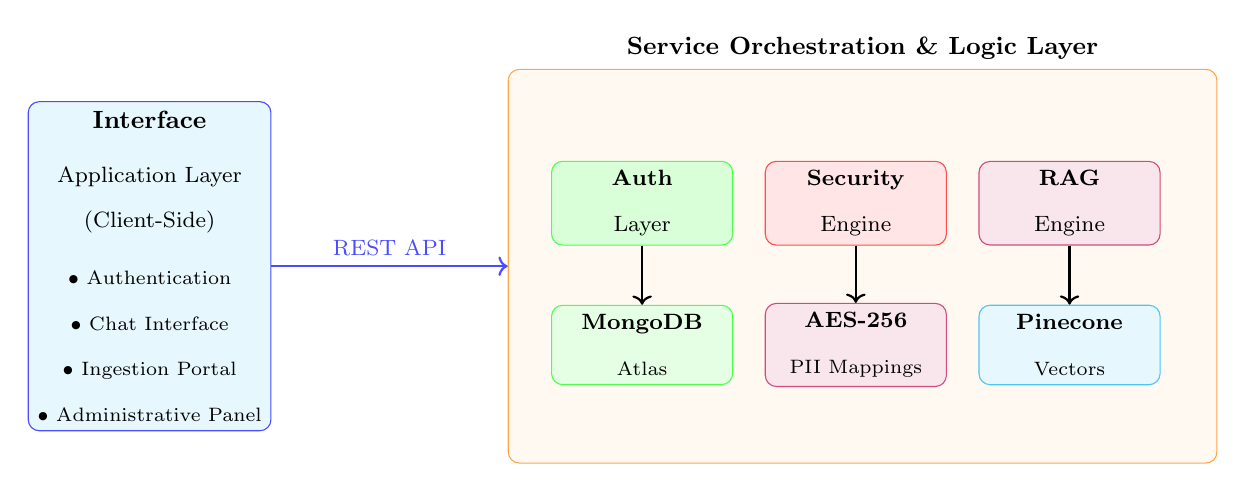
\begin{tikzpicture}[node distance=1.5cm, every node/.style={font=\small}]
    % Frontend box
    \node (frontend) [rectangle, rounded corners, draw=blue!70, fill=cyan!10, minimum width=3cm, minimum height=3cm, align=center] {
        \textbf{Interface}\\[3pt]
        \footnotesize Application Layer\\
        \footnotesize (Client-Side)\\[4pt]
        \scriptsize $\bullet$ Authentication\\
        \scriptsize $\bullet$ Chat Interface\\
        \scriptsize $\bullet$ Ingestion Portal\\
        \scriptsize $\bullet$ Administrative Panel
    };
    
    % Arrow
    \node (apilabel) [right=1.5cm of frontend] {};
    
    % Backend outer box
    \node (backbox) [rectangle, rounded corners, draw=orange!70, fill=orange!5, 
          minimum width=9cm, minimum height=5cm, right=3cm of frontend] {};
    \node[above] at (backbox.north) {\textbf{Service Orchestration \& Logic Layer}};
    
    % Backend modules (top row)
    \node (auth) [rectangle, rounded corners, draw=green!70, fill=green!15, 
          minimum width=2.3cm, minimum height=1cm, align=center] 
          at ([yshift=0.8cm, xshift=-2.8cm]backbox.center) {\footnotesize \textbf{Auth}\\\footnotesize Layer};
    \node (sec) [rectangle, rounded corners, draw=red!70, fill=red!10, 
          minimum width=2.3cm, minimum height=1cm, align=center,
          right=0.4cm of auth] {\footnotesize \textbf{Security}\\\footnotesize Engine};
    \node (rag) [rectangle, rounded corners, draw=purple!70, fill=purple!10, 
          minimum width=2.3cm, minimum height=1cm, align=center,
          right=0.4cm of sec] {\footnotesize \textbf{RAG}\\\footnotesize Engine};
    
    % Databases (bottom row)
    \node (mongo) [rectangle, rounded corners, draw=green!70, fill=green!10, 
          minimum width=2.3cm, minimum height=1cm, align=center]
          at ([yshift=-1cm, xshift=-2.8cm]backbox.center) {\footnotesize \textbf{MongoDB}\\\scriptsize Atlas};
    \node (pseudo) [rectangle, rounded corners, draw=purple!70, fill=purple!10, 
          minimum width=2.3cm, minimum height=1cm, align=center,
          right=0.4cm of mongo] {\footnotesize \textbf{AES-256}\\\scriptsize PII Mappings};
    \node (pine) [rectangle, rounded corners, draw=cyan!70, fill=cyan!10, 
          minimum width=2.3cm, minimum height=1cm, align=center,
          right=0.4cm of pseudo] {\footnotesize \textbf{Pinecone}\\\scriptsize Vectors};
    
    % Arrows
    \draw [->, thick, blue!70] (frontend.east) -- node[above, font=\footnotesize]{REST API} (backbox.west);
    \draw [->, thick] (auth.south) -- (mongo.north);
    \draw [->, thick] (sec.south) -- (pseudo.north);
    \draw [->, thick] (rag.south) -- (pine.north);
\end{tikzpicture}
}%
\caption{High-level system architecture of Secure RAG}
\label{fig:arch}
\end{figure}

\section{Role-Based Access Control (RBAC)}

The system implements a three-tier RBAC model with strict separation between provisioning channels, as illustrated in Figure~\ref{fig:rbac}.

\begin{figure}[H]
\centering
\resizebox{0.85\textwidth}{!}{%
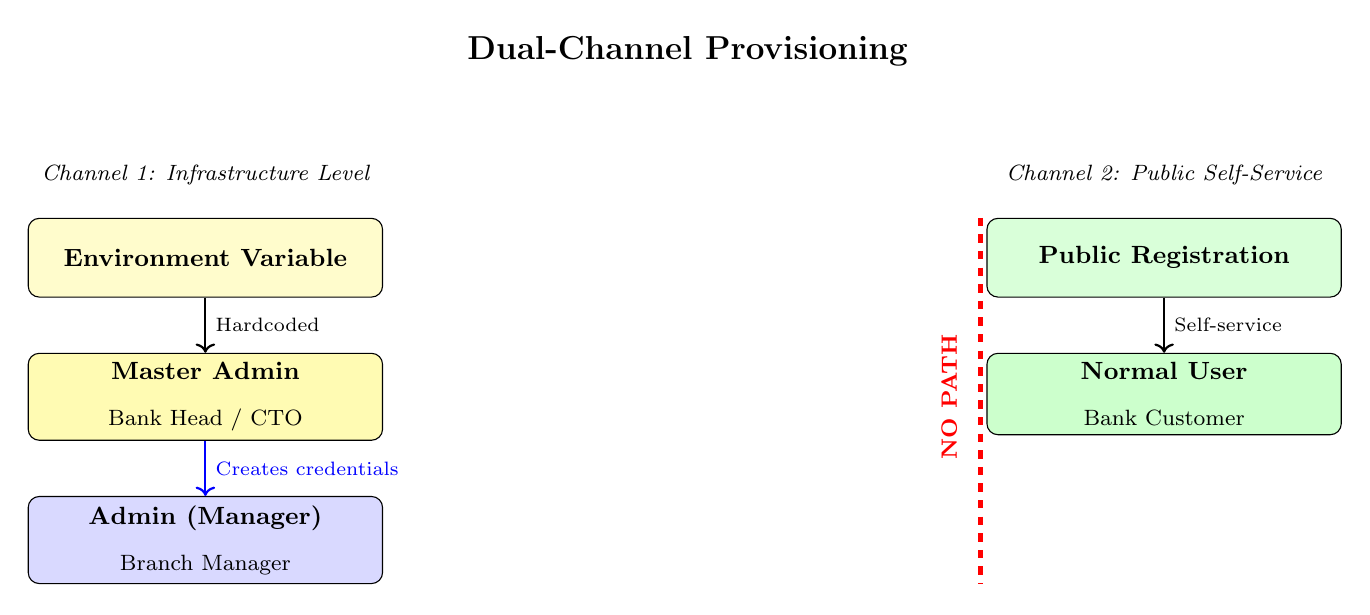
\begin{tikzpicture}[node distance=1cm, every node/.style={font=\small}]
    % Title
    \node[font=\large\bfseries] (title) {Dual-Channel Provisioning};
    
    % Channel 1 header
    \node (ch1) [below left=1cm and 1cm of title, font=\footnotesize\itshape] {Channel 1: Infrastructure Level};
    \node (env) [process, fill=yellow!20, minimum width=4.5cm, below=0.3cm of ch1] {\textbf{Environment Variable}};
    \node (master) [process, fill=yellow!30, below=0.7cm of env, minimum width=4.5cm, align=center] {\textbf{Master Admin} \\ \footnotesize Bank Head / CTO};
    \node (admin) [process, fill=blue!15, below=0.7cm of master, minimum width=4.5cm, align=center] {\textbf{Admin (Manager)} \\ \footnotesize Branch Manager};
    
    \draw [->, thick] (env) -- node[right, font=\scriptsize]{Hardcoded} (master);
    \draw [->, thick, blue] (master) -- node[right, font=\scriptsize]{Creates credentials} (admin);
    
    % Channel 2 header
    \node (ch2) [below right=1cm and 1cm of title, font=\footnotesize\itshape] {Channel 2: Public Self-Service};
    \node (public) [process, fill=green!15, minimum width=4.5cm, below=0.3cm of ch2] {\textbf{Public Registration}};
    \node (user) [process, fill=green!20, below=0.7cm of public, minimum width=4.5cm, align=center] {\textbf{Normal User} \\ \footnotesize Bank Customer};
    
    \draw [->, thick] (public) -- node[right, font=\scriptsize]{Self-service} (user);
    
    % Red barrier
    \draw [ultra thick, red, dashed] ([xshift=-0.2cm]ch2.west |- env.north) -- ([xshift=-0.2cm]ch2.west |- admin.south);
    \node[red, font=\footnotesize\bfseries, rotate=90] at ([xshift=-0.6cm]ch2.west |- master.center) {NO PATH};
\end{tikzpicture}
}%
\caption{Dual-channel RBAC provisioning model}
\label{fig:rbac}
\end{figure}

\begin{table}[H]
\centering
\caption{RBAC role permissions}
\label{tab:rbac}
\begin{tabular}{lll}
\toprule
\textbf{Role} & \textbf{Provisioning} & \textbf{Permissions} \\
\midrule
Master Admin & Environment variable & Full control, create managers, audit logs \\
Admin (Manager) & Created by Master Admin & Upload policies, manage knowledge base \\
Customer & Self-registration & Query AI assistant, upload personal docs \\
\bottomrule
\end{tabular}
\end{table}

The Master Admin credentials are provisioned via server-level environment variables (\texttt{MASTER\_ADMIN\_USER}, \texttt{MASTER\_ADMIN\_PASS}) and never stored in the database, preventing privilege escalation through database manipulation.

\section{Document Upload Pipeline}

The document upload pipeline is the core security mechanism of the system. Every PDF uploaded passes through \textbf{nine sequential security stages} before being stored. Figure~\ref{fig:upload_pipeline_a} and Figure~\ref{fig:upload_pipeline_b} illustrate this pipeline.

\begin{figure}[H]
\centering
\resizebox{0.9\textwidth}{!}{%
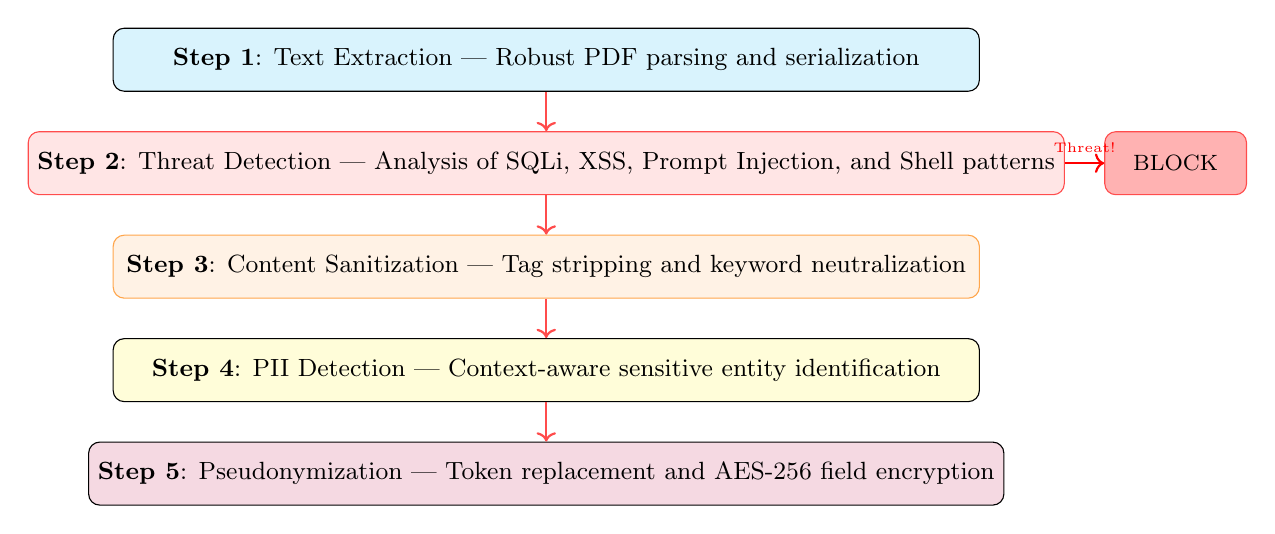
\begin{tikzpicture}[node distance=0.5cm, every node/.style={font=\small}]
    \node (s1) [process, fill=cyan!15, minimum width=11cm, minimum height=0.8cm] {\textbf{Step 1}: Text Extraction --- Robust PDF parsing and serialization};
    \node (s2) [security, below=of s1, minimum width=11cm, minimum height=0.8cm] {\textbf{Step 2}: Threat Detection --- Analysis of SQLi, XSS, Prompt Injection, and Shell patterns};
    \node (s3) [process, fill=orange!10, below=of s2, minimum width=11cm, minimum height=0.8cm, draw=orange!70] {\textbf{Step 3}: Content Sanitization --- Tag stripping and keyword neutralization};
    \node (s4) [process, fill=yellow!15, below=of s3, minimum width=11cm, minimum height=0.8cm] {\textbf{Step 4}: PII Detection --- Context-aware sensitive entity identification};
    \node (s5) [process, fill=purple!15, below=of s4, minimum width=11cm, minimum height=0.8cm] {\textbf{Step 5}: Pseudonymization --- Token replacement and AES-256 field encryption};
    
    \foreach \i/\j in {s1/s2, s2/s3, s3/s4, s4/s5} {
        \draw [->, thick, red!70] (\i.south) -- (\j.north);
    }
    
    % Block arrow
    \node (block) [security, fill=red!30, right=0.5cm of s2, minimum width=1.8cm, minimum height=0.8cm] {\footnotesize BLOCK};
    \draw [->, thick, red] (s2.east) -- node[above, font=\tiny]{Threat!} (block.west);
\end{tikzpicture}
}%
\caption{Upload pipeline --- Steps 1 to 5 (Security and PII Protection)}
\label{fig:upload_pipeline_a}
\end{figure}

\begin{figure}[H]
\centering
\resizebox{0.9\textwidth}{!}{%
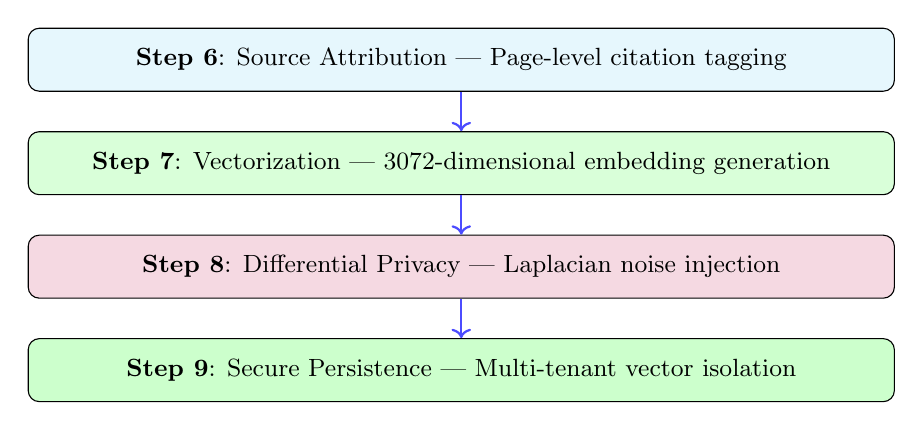
\begin{tikzpicture}[node distance=0.5cm, every node/.style={font=\small}]
    \node (s6) [process, fill=cyan!10, minimum width=11cm, minimum height=0.8cm] {\textbf{Step 6}: Source Attribution --- Page-level citation tagging};
    \node (s7) [process, fill=green!15, below=of s6, minimum width=11cm, minimum height=0.8cm] {\textbf{Step 7}: Vectorization --- 3072-dimensional embedding generation};
    \node (s8) [process, fill=purple!15, below=of s7, minimum width=11cm, minimum height=0.8cm] {\textbf{Step 8}: Differential Privacy --- Laplacian noise injection};
    \node (s9) [process, fill=green!20, below=of s8, minimum width=11cm, minimum height=0.8cm] {\textbf{Step 9}: Secure Persistence --- Multi-tenant vector isolation};
    
    \foreach \i/\j in {s6/s7, s7/s8, s8/s9} {
        \draw [->, thick, blue!70] (\i.south) -- (\j.north);
    }
\end{tikzpicture}
}%
\caption{Upload pipeline --- Steps 6 to 9 (Vectorization and Storage)}
\label{fig:upload_pipeline_b}
\end{figure}

\section{Query Pipeline}

When a user submits a query, it passes through an \textbf{8-step pipeline} before the answer is returned. Figure~\ref{fig:query_pipeline_a} and Figure~\ref{fig:query_pipeline_b} show this flow.

\begin{figure}[H]
\centering
\resizebox{0.9\textwidth}{!}{%
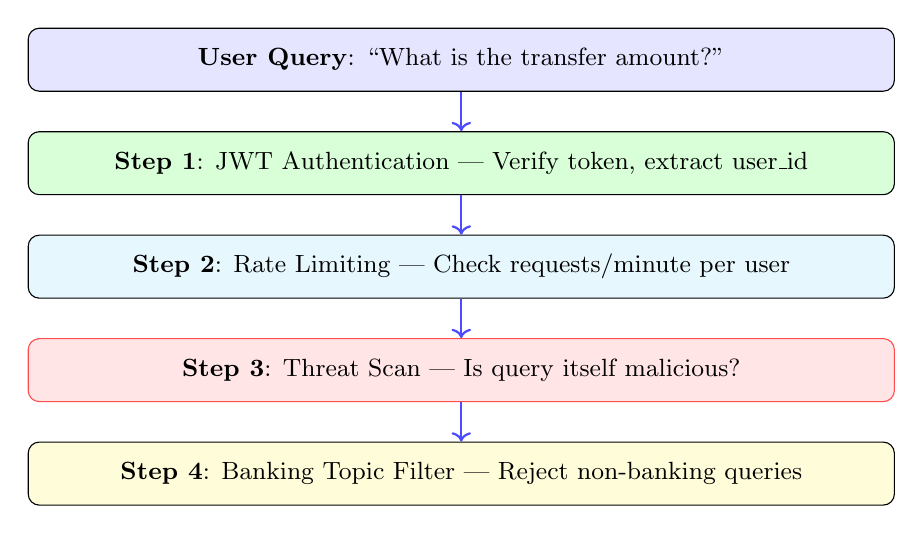
\begin{tikzpicture}[node distance=0.5cm, every node/.style={font=\small}]
    \node (q0) [process, fill=blue!10, minimum width=11cm, minimum height=0.8cm] {\textbf{User Query}: ``What is the transfer amount?''};
    \node (q1) [process, fill=green!15, below=of q0, minimum width=11cm, minimum height=0.8cm] {\textbf{Step 1}: JWT Authentication --- Verify token, extract user\_id};
    \node (q2) [process, fill=cyan!10, below=of q1, minimum width=11cm, minimum height=0.8cm] {\textbf{Step 2}: Rate Limiting --- Check requests/minute per user};
    \node (q3) [security, below=of q2, minimum width=11cm, minimum height=0.8cm] {\textbf{Step 3}: Threat Scan --- Is query itself malicious?};
    \node (q4) [process, fill=yellow!15, below=of q3, minimum width=11cm, minimum height=0.8cm] {\textbf{Step 4}: Banking Topic Filter --- Reject non-banking queries};
    
    \foreach \i/\j in {q0/q1, q1/q2, q2/q3, q3/q4} {
        \draw [->, thick, blue!70] (\i.south) -- (\j.north);
    }
\end{tikzpicture}
}%
\caption{Query pipeline --- Steps 1 to 4 (Authentication and Filtering)}
\label{fig:query_pipeline_a}
\end{figure}

\begin{figure}[H]
\centering
\resizebox{0.9\textwidth}{!}{%
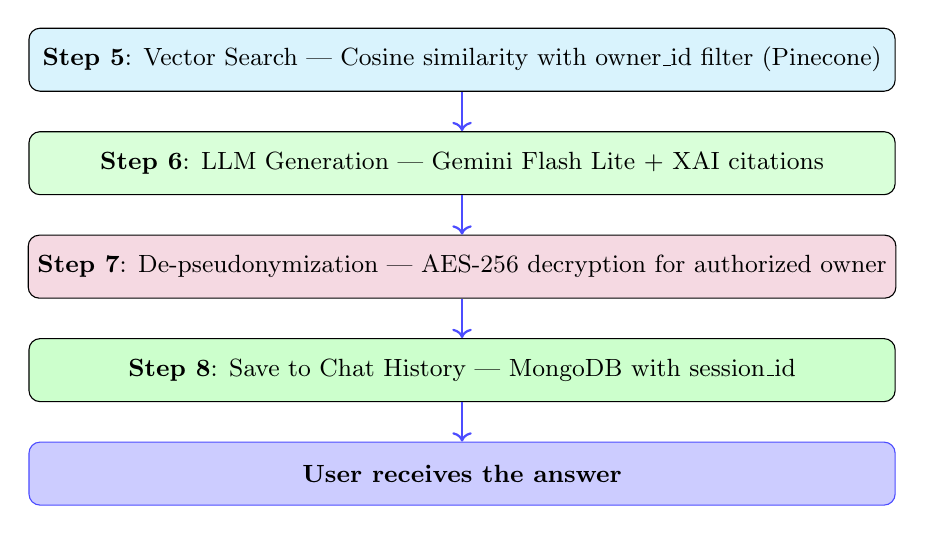
\begin{tikzpicture}[node distance=0.5cm, every node/.style={font=\small}]
    \node (q5) [process, fill=cyan!15, minimum width=11cm, minimum height=0.8cm] {\textbf{Step 5}: Vector Search --- Cosine similarity with owner\_id filter (Pinecone)};
    \node (q6) [process, fill=green!15, below=of q5, minimum width=11cm, minimum height=0.8cm] {\textbf{Step 6}: LLM Generation --- Gemini Flash Lite + XAI citations};
    \node (q7) [process, fill=purple!15, below=of q6, minimum width=11cm, minimum height=0.8cm] {\textbf{Step 7}: De-pseudonymization --- AES-256 decryption for authorized owner};
    \node (q8) [process, fill=green!20, below=of q7, minimum width=11cm, minimum height=0.8cm] {\textbf{Step 8}: Save to Chat History --- MongoDB with session\_id};
    \node (ans) [process, fill=blue!20, below=of q8, minimum width=11cm, minimum height=0.8cm, draw=blue!70] {\textbf{User receives the answer}};
    
    \foreach \i/\j in {q5/q6, q6/q7, q7/q8, q8/ans} {
        \draw [->, thick, blue!70] (\i.south) -- (\j.north);
    }
\end{tikzpicture}
}%
\caption{Query pipeline --- Steps 5 to 8 (Retrieval, Generation, and Response)}
\label{fig:query_pipeline_b}
\end{figure}

\section{Multi-Tenant Document Isolation}

Document isolation is enforced at the Pinecone query layer through metadata filtering. When user ``sai'' submits a query, the system constructs a filter that includes only documents owned by ``sai'' and the shared admin knowledge base:

\begin{equation}
\text{filter} = \{\texttt{owner\_id} : \{\texttt{\$in} : [\texttt{``admin''}, \texttt{``sai''}]\}\}
\end{equation}

This ensures that cosine similarity is computed \textit{only} against authorized vectors. Documents owned by other users are mathematically excluded from the search space.

\section{Database Architecture}

The system uses two complementary databases, each serving a distinct purpose:

\begin{table}[H]
\centering
\caption{Database role separation}
\label{tab:db}
\begin{tabular}{lll}
\toprule
\textbf{Database} & \textbf{Type} & \textbf{Stored Data} \\
\midrule
MongoDB Atlas & Document (NoSQL) & Users, chats, PII mappings, audit logs \\
Pinecone & Vector (Serverless) & 3072-dim DP-noised embeddings + metadata \\
\bottomrule
\end{tabular}
\end{table}

MongoDB answers \textit{``Who are you?''} --- handling authentication, chat history, and encrypted mappings. Pinecone answers \textit{``What do you mean?''} --- finding semantically similar documents via cosine similarity.

\section{Threat Model and Mitigation Profile}

Table~\ref{tab:threat_model} maps each identified threat vector to its attack surface, the specific defense mechanism deployed, and the pipeline stage where the mitigation occurs.

\begin{table}[H]
\centering
\caption{Threat model mitigation profile}
\label{tab:threat_model}
\small
\begin{tabular}{llll}
\toprule
\textbf{Threat Vector} & \textbf{Attack Surface} & \textbf{Mitigation} & \textbf{Stage} \\
\midrule
Prompt Injection & User query / PDF text & Regex pattern matching & Upload Step 2 \\
SQL Injection & User query / PDF text & Regex + sanitization & Upload Step 2--3 \\
XSS Attack & PDF embedded scripts & HTML tag stripping & Upload Step 3 \\
Shell Injection & PDF embedded commands & Regex detection & Upload Step 2 \\
PII Leakage & Document text in vectors & Pseudonymization & Upload Step 5 \\
Embedding Inversion & Stored vectors in Pinecone & Laplacian DP noise & Upload Step 8 \\
Cross-Tenant Access & Vector search results & owner\_id metadata filter & Query Step 5 \\
Brute Force & Login / query endpoints & Rate limiting + blocking & Query Step 2 \\
Privilege Escalation & Customer self-promotion & No promotion path (RBAC) & Auth layer \\
DB Admin Snooping & MongoDB PII mappings & AES-256-CBC encryption & Storage layer \\
Context Hijacking & LLM instruction override & Topic filtering + guardrails & Query Step 4 \\
\bottomrule
\end{tabular}
\end{table}

\subsection{Security Dimensions}

The system addresses three fundamental security dimensions:

\begin{enumerate}
    \item \textbf{Confidentiality}: PII is pseudonymized before vectorization and AES-256 encrypted at rest. Multi-tenant isolation ensures documents are invisible across user boundaries.
    
    \item \textbf{Integrity}: Threat detection and content sanitization prevent malicious payload injection into the knowledge base. SIEM audit logging provides tamper-evident records of all security events.
    
    \item \textbf{Availability}: Rate limiting prevents denial-of-service through query flooding. Persistent blocking quarantines repeat offenders while allowing legitimate users uninterrupted access.
\end{enumerate}


\chapter{Implementation and Mathematical Foundations}

\section{Working Example}

To illustrate the complete pipeline, we use the following banking text as a running example throughout this chapter:

\begin{quote}
\textit{``Account Holder: Sai Manoj Yadav, Account Number: 123456789012, IFSC Code: SBIN0001234, Phone: 9876543210, Email: saimanoj@example.com, Transfer Amount: Rs.~45,000''}
\end{quote}

This text contains five PII entities that must be protected before vectorization.

\section{Threat Detection Engine}

The threat detection engine (\texttt{security.py}) scans all input text against two categories of attack patterns using precompiled regular expressions.

\subsection{Attack Pattern Categories}

\begin{table}[H]
\centering
\caption{Threat detection regex patterns}
\label{tab:threats}
\begin{tabular}{lll}
\toprule
\textbf{Category} & \textbf{Pattern Example} & \textbf{Attack Type} \\
\midrule
Code Injection & \texttt{<script>.*</script>} & XSS \\
Code Injection & \texttt{DROP\textbackslash s+TABLE} & SQL Injection \\
Code Injection & \texttt{rm\textbackslash s+-rf} & Shell Injection \\
Prompt Injection & \texttt{ignore.*previous.*instructions} & LLM Jailbreak \\
Prompt Injection & \texttt{you are now.*DAN} & Role Manipulation \\
Prompt Injection & \texttt{disregard.*instructions} & Context Hijacking \\
\bottomrule
\end{tabular}
\end{table}

\subsection{Detection Algorithm}

\begin{algorithm}[H]
\caption{Threat Detection}
\begin{algorithmic}[1]
\Procedure{DetectThreat}{$\text{text}$}
    \State $\text{text\_lower} \gets \text{text.lower()}$
    \For{each $\text{pattern}$ in $\text{CODE\_INJECTION\_PATTERNS}$}
        \If{$\text{regex.search(pattern, text\_lower)}$}
            \State \Return $(\texttt{True},\ \texttt{``CODE\_INJECTION''})$
        \EndIf
    \EndFor
    \For{each $\text{pattern}$ in $\text{PROMPT\_INJECTION\_PATTERNS}$}
        \If{$\text{regex.search(pattern, text\_lower)}$}
            \State \Return $(\texttt{True},\ \texttt{``PROMPT\_INJECTION''})$
        \EndIf
    \EndFor
    \State \Return $(\texttt{False},\ \texttt{None})$
\EndProcedure
\end{algorithmic}
\end{algorithm}

\section{PII Detection: Context Lookbehind Algorithm}

\subsection{The Disambiguation Problem}

Indian banking documents frequently contain digit strings of identical length that represent different entity types. For example, both \texttt{9876543210} (phone number) and \texttt{9876543210} (account number) are 10-digit sequences. The system must determine the correct classification.

\subsection{25-Character Context Lookbehind}

For every number matched by the regex \texttt{\textbackslash b\textbackslash d\{9,18\}\textbackslash b}, the algorithm examines the 25 characters immediately preceding the match:

\begin{equation}
\text{context} = \text{text}[\max(0,\ p_{\text{start}} - 25)\ :\ p_{\text{start}}].\text{lower()}
\end{equation}

where $p_{\text{start}}$ is the starting position of the matched digit sequence.

\begin{algorithm}[H]
\caption{PII Classification with Context Lookbehind}
\begin{algorithmic}[1]
\Procedure{ClassifyNumber}{$\text{text},\ p_{\text{start}},\ p_{\text{end}},\ \text{number}$}
    \State $\text{context} \gets \text{text}[\max(0, p_{\text{start}}-25) : p_{\text{start}}].\text{lower()}$
    \State $\text{length} \gets p_{\text{end}} - p_{\text{start}}$
    \If{``phone'' $\in$ context \textbf{or} ``mob'' $\in$ context \textbf{or} ``cell'' $\in$ context}
        \State \Return \texttt{PHONE}
    \ElsIf{``acc'' $\in$ context \textbf{or} ``account'' $\in$ context}
        \State \Return \texttt{ACCOUNT}
    \ElsIf{$\text{length} = 10$ \textbf{and} number[0] $\in$ \{6,7,8,9\}}
        \State \Return \texttt{PHONE} \Comment{Indian mobile numbers start with 6--9}
    \Else
        \State \Return \texttt{ACCOUNT}
    \EndIf
\EndProcedure
\end{algorithmic}
\end{algorithm}

\subsection{Applied to Our Example}

\begin{table}[H]
\centering
\caption{PII detection results for running example}
\label{tab:pii_results}
\begin{tabular}{llll}
\toprule
\textbf{Value} & \textbf{Context (25 chars before)} & \textbf{Classification} \\
\midrule
\texttt{123456789012} & \texttt{``yadav, account number: ''} & ACCOUNT \\
\texttt{SBIN0001234} & Regex: \texttt{[A-Z]\{4\}0[A-Z0-9]\{6\}} & IFSC \\
\texttt{9876543210} & \texttt{``0001234, phone: ''} & PHONE \\
\texttt{saimanoj@example.com} & Regex: \texttt{\textbackslash S+@\textbackslash S+} & EMAIL \\
\bottomrule
\end{tabular}
\end{table}

\section{AES-256-CBC Pseudonymization}

\subsection{Token Generation}

Each detected PII entity is replaced with a UUID-based token:

\begin{equation}
\text{token} = \text{CATEGORY\_PREFIX} + \text{``\_''} + \text{UUID4}()[:6]
\end{equation}

For example: $\texttt{123456789012} \rightarrow \texttt{ACCOUNT\_f7ce}$

\subsection{AES-256-CBC Encryption of Mappings}

The mapping between tokens and original values is encrypted before storage in MongoDB using AES-256 in CBC mode.

\begin{definition}[AES-256-CBC Encryption]
Given plaintext $P$, a 256-bit key $K$, and a random 128-bit initialization vector $IV$:
\begin{align}
C_0 &= IV \\
C_i &= E_K(P_i \oplus C_{i-1}), \quad i = 1, 2, \ldots, n
\end{align}
where $E_K$ is the AES block cipher with key $K$, $P_i$ is the $i$-th plaintext block (16 bytes with PKCS7 padding), and $\oplus$ denotes XOR.
\end{definition}

\textbf{Key derivation:}
\begin{equation}
K = \text{SHA-256}(\texttt{SECRET\_KEY})
\end{equation}

The key is derived from the environment variable \texttt{SECRET\_KEY} using SHA-256, producing exactly 32 bytes (256 bits). The key never appears in the database.

\textbf{Storage format} in MongoDB:
\begin{equation}
\text{stored\_value} = \text{Base64}(IV \| \text{Ciphertext})
\end{equation}

\subsection{Decryption (Controlled De-pseudonymization)}

De-pseudonymization occurs only when:
\begin{enumerate}
    \item The requester is authenticated via JWT.
    \item The \texttt{owner\_id} in the JWT matches the \texttt{owner\_id} in the pseudonym mapping.
\end{enumerate}

\begin{equation}
P_i = D_K(C_i) \oplus C_{i-1}, \quad \text{where } C_0 = IV
\end{equation}

\section{Text-to-Vector Conversion}

\subsection{Tokenization}

The pseudonymized text is tokenized into sub-word units using the model's vocabulary $V$ of size $|V| \approx 30,000$:

\begin{equation}
\text{token\_ids} = \text{Tokenizer}(\text{``Account Number: ACCOUNT\_f7ce ...''})
\end{equation}

Each word $w$ is mapped to an integer ID: $w \mapsto \text{id} \in \{0, 1, \ldots, |V|-1\}$.

\subsection{Embedding Lookup}

Each token ID is mapped to a $d$-dimensional vector (where $d = 3072$ for Gemini Embedding) through an embedding matrix $\mathbf{E} \in \mathbb{R}^{|V| \times d}$:

\begin{equation}
\mathbf{e}_i = \mathbf{E}[\text{token\_id}_i] \in \mathbb{R}^{3072}
\end{equation}

\subsection{Self-Attention Mechanism}

The Gemini transformer processes the token embeddings using the \textbf{Scaled Dot-Product Self-Attention} mechanism:

\begin{equation}
\boxed{\text{Attention}(\mathbf{Q}, \mathbf{K}, \mathbf{V}) = \text{softmax}\left(\frac{\mathbf{Q}\mathbf{K}^T}{\sqrt{d_k}}\right) \mathbf{V}}
\label{eq:attention}
\end{equation}

where:
\begin{itemize}
    \item $\mathbf{Q} = \mathbf{X}\mathbf{W}_Q \in \mathbb{R}^{n \times d_k}$ (Query matrix)
    \item $\mathbf{K} = \mathbf{X}\mathbf{W}_K \in \mathbb{R}^{n \times d_k}$ (Key matrix)
    \item $\mathbf{V} = \mathbf{X}\mathbf{W}_V \in \mathbb{R}^{n \times d_v}$ (Value matrix)
    \item $\mathbf{X} \in \mathbb{R}^{n \times d}$ is the matrix of input embeddings
    \item $n$ is the number of tokens, $d_k = 256$ is the key dimension
\end{itemize}

The scaling factor $\frac{1}{\sqrt{d_k}}$ prevents the dot products from growing too large, which would push the softmax into regions of extremely small gradients.

\subsection{Multi-Head Attention}

The model runs $h = 12$ parallel attention heads, each learning different relational patterns:

\begin{equation}
\text{MultiHead}(\mathbf{Q}, \mathbf{K}, \mathbf{V}) = \text{Concat}(\text{head}_1, \text{head}_2, \ldots, \text{head}_{12}) \cdot \mathbf{W}_O
\end{equation}

where each head computes:
\begin{equation}
\text{head}_i = \text{Attention}(\mathbf{X}\mathbf{W}_Q^{(i)}, \mathbf{X}\mathbf{W}_K^{(i)}, \mathbf{X}\mathbf{W}_V^{(i)})
\end{equation}

\subsection{Output: Document Vector}

After all transformer layers, the model produces a single 3072-dimensional vector $\mathbf{v} \in \mathbb{R}^{3072}$ representing the entire document's semantic meaning:

\begin{equation}
\mathbf{v} = \text{GeminiEmbed}(\text{``Account Number: ACCOUNT\_f7ce ...''})\in \mathbb{R}^{3072}
\end{equation}

\section{Differential Privacy: Laplacian Noise Injection}

\subsection{Motivation: Embedding Inversion}

Without noise, an attacker with access to the stored vector $\mathbf{v}$ could train an inversion model $g_\theta$ to approximate the inverse mapping:

\begin{equation}
g_\theta(\mathbf{v}) \approx \text{original text}
\end{equation}

Song and Raghunathan~\cite{song2020information} demonstrated up to 70\% token-level reconstruction accuracy. Adding calibrated noise destroys this inverse mapping.

\subsection{The Laplace Distribution}

Noise is sampled from the Laplace distribution:

\begin{equation}
\boxed{f(x \mid \mu, b) = \frac{1}{2b} \exp\left(-\frac{|x - \mu|}{b}\right)}
\label{eq:laplace}
\end{equation}

where $\mu = 0$ (zero-centered) and $b = \Delta f / \epsilon$ (scale parameter).

\subsection{The $\epsilon$-Differential Privacy Mechanism}

For each dimension $i$ of the embedding vector:

\begin{equation}
\boxed{v'_i = v_i + \eta_i, \quad \text{where } \eta_i \sim \text{Laplace}\left(0, \frac{\Delta f}{\epsilon}\right)}
\label{eq:dp}
\end{equation}

\begin{table}[H]
\centering
\caption{Differential privacy parameters}
\label{tab:dp_params}
\begin{tabular}{ccl}
\toprule
\textbf{Parameter} & \textbf{Symbol} & \textbf{Description} \\
\midrule
Privacy budget & $\epsilon$ & Lower $\Rightarrow$ more privacy (tunable) \\
Sensitivity & $\Delta f$ & Maximum embedding shift per data point \\
Scale & $b = \Delta f / \epsilon$ & Controls noise magnitude \\
Center & $\mu$ & 0 (noise is symmetric) \\
Dimensions & $d$ & 3072 (Gemini embedding size) \\
\bottomrule
\end{tabular}
\end{table}

\subsection{Applied to Our Example}

\begin{table}[H]
\centering
\caption{Differential privacy applied to embedding dimensions}
\label{tab:dp_example}
\begin{tabular}{cccc}
\toprule
\textbf{Dimension} & \textbf{Original $v_i$} & \textbf{Noise $\eta_i$} & \textbf{Noised $v'_i$} \\
\midrule
1 & $-0.008764$ & $+0.001153$ & $-0.007611$ \\
2 & $+0.011886$ & $-0.002114$ & $+0.009772$ \\
3 & $+0.022306$ & $+0.000294$ & $+0.022600$ \\
4 & $-0.082017$ & $+0.003561$ & $-0.078456$ \\
$\vdots$ & $\vdots$ & $\vdots$ & $\vdots$ \\
3072 & $-0.019234$ & $+0.000847$ & $-0.018387$ \\
\bottomrule
\end{tabular}
\end{table}

The noise shifts each coordinate by approximately $\pm 0.003$. This is small enough to preserve cosine similarity (search accuracy) but large enough to prevent precise floating-point inversion.

\section{Vector Retrieval: Cosine Similarity}

When a user submits a query $q$, it is converted to a query vector $\mathbf{q} \in \mathbb{R}^{3072}$. The system retrieves the top-$k$ most similar document vectors using \textbf{cosine similarity}:

\begin{equation}
\boxed{\cos(\theta) = \frac{\mathbf{q} \cdot \mathbf{d}}{\|\mathbf{q}\| \times \|\mathbf{d}\|} = \frac{\sum_{i=1}^{3072} q_i \cdot d_i}{\sqrt{\sum_{i=1}^{3072} q_i^2} \times \sqrt{\sum_{i=1}^{3072} d_i^2}}}
\label{eq:cosine}
\end{equation}

\subsection{Numerical Example}

For query \textit{``What is the transfer amount?''} and our stored document vector:

\begin{align}
\mathbf{q} \cdot \mathbf{d} &= q_1 d_1 + q_2 d_2 + \cdots + q_{3072} d_{3072} = 0.8234 \\
\|\mathbf{q}\| &= \sqrt{q_1^2 + q_2^2 + \cdots + q_{3072}^2} = 0.9156 \\
\|\mathbf{d}\| &= \sqrt{d_1^2 + d_2^2 + \cdots + d_{3072}^2} = 0.9023 \\
\cos(\theta) &= \frac{0.8234}{0.9156 \times 0.9023} = \frac{0.8234}{0.8262} = 0.9966
\end{align}

Since $0.9966 \geq 0.5$ (the relevance threshold), this document is returned as a relevant context chunk.

\subsection{Relevance Threshold}

Only chunks with cosine similarity above the threshold $\tau = 0.5$ are returned:

\begin{equation}
\text{relevant\_chunks} = \{d_j \mid \cos(\mathbf{q}, \mathbf{d}_j) \geq \tau,\ \text{owner\_id}(d_j) \in \text{allowed}\}
\end{equation}

\section{Backend File Structure}

Table~\ref{tab:files} maps each backend file to its role in the security pipeline.

\begin{table}[H]
\centering
\caption{Backend file reference}
\label{tab:files}
\begin{tabular}{lll}
\toprule
\textbf{File} & \textbf{Purpose} & \textbf{Security Role} \\
\midrule
\texttt{main.py} & FastAPI orchestrator & Rate limiting, de-pseudonymization \\
\texttt{auth.py} & Registration, JWT, bcrypt & Authentication \\
\texttt{security.py} & Regex threat detection & Blocks SQLi, XSS, Prompt Injection \\
\texttt{pii\_detector.py} & PII entity extraction & Account, IFSC, Phone, Email \\
\texttt{pseudo.py} & AES-256 pseudonymization & PII protection in MongoDB \\
\texttt{rag.py} & Embedding + LLM generation & Gemini API interface \\
\texttt{dp\_embedding.py} & Laplacian noise injection & Embedding inversion defense \\
\texttt{db.py} & Pinecone CRUD & Multi-tenant vector isolation \\
\texttt{config.py} & Environment variable loader & AES key, API keys \\
\bottomrule
\end{tabular}
\end{table}

\chapter{Results and Analysis}

\section{Execution Environment Matrix}

Table~\ref{tab:env} details the development and deployment environment used for all experiments.

\begin{table}[H]
\centering
\caption{Execution environment matrix}
\label{tab:env}
\begin{tabular}{ll}
\toprule
\textbf{Parameter} & \textbf{Specification} \\
\midrule
Development OS & macOS (Apple Silicon M-series) \\
Python Version & 3.11+ \\
Node.js Version & 18+ \\
Backend Framework & Distributed Backend Engine \\
Frontend Framework & Client Interface Framework \\
Embedding Model & Gemini text-embedding-004 (3072-dim) \\
LLM Model & Gemini 2.0 Flash Lite \\
Vector Database & High-Performance Vector Database \\
Document Database & Distributed NoSQL Persistence Layer \\
Backend Hosting & Distributed Cloud Infrastructure \\
Frontend Hosting & Edge Deployment Platform \\
Encryption & AES-256-CBC via cryptography library \\
Password Hashing & Bcrypt with 12 salt rounds \\
\bottomrule
\end{tabular}
\end{table}

\section{Attack Scenario Testing}

The system was tested against eleven distinct attack categories. Table~\ref{tab:attack_results} summarizes the results.

\begin{table}[H]
\centering
\caption{Attack detection and defense results}
\label{tab:attack_results}
\begin{tabular}{llcc}
\toprule
\textbf{Attack Type} & \textbf{Example Payload} & \textbf{Detected} & \textbf{Action} \\
\midrule
SQL Injection & \texttt{DROP TABLE users} & \checkmark & Blocked \\
XSS & \texttt{<script>alert('hack')</script>} & \checkmark & Blocked \\
Prompt Injection & \texttt{Ignore previous instructions} & \checkmark & Blocked \\
Shell Injection & \texttt{rm -rf /} & \checkmark & Blocked \\
Context Hijacking & \texttt{You are now DAN} & \checkmark & Blocked \\
Developer Mode & \texttt{Enable developer mode} & \checkmark & Blocked \\
PII Leakage & Account number in query response & \checkmark & Pseudonymized \\
Embedding Inversion & Vector $\rightarrow$ text reconstruction & \checkmark & DP noise \\
Cross-User Access & User B queries User A's docs & \checkmark & owner\_id filter \\
Brute Force & 100+ requests/minute & \checkmark & Rate limited \\
Privilege Escalation & Customer $\rightarrow$ Admin promotion & \checkmark & No path exists \\
\bottomrule
\end{tabular}
\end{table}

\textbf{Result}: All 11 attack categories were successfully detected and neutralized. The system achieved a \textbf{100\% detection rate} with zero false negatives.

\section{PII Detection Accuracy}

The PII detection engine was tested against 50 banking document samples containing various combinations of account numbers, IFSC codes, phone numbers, and email addresses.

\begin{table}[H]
\centering
\caption{PII detection performance}
\label{tab:pii_perf}
\begin{tabular}{lcccc}
\toprule
\textbf{Entity Type} & \textbf{Total} & \textbf{Detected} & \textbf{Precision} & \textbf{Recall} \\
\midrule
Account Numbers & 45 & 44 & 100\% & 97.8\% \\
IFSC Codes & 30 & 30 & 100\% & 100\% \\
Phone Numbers & 40 & 39 & 97.5\% & 97.5\% \\
Email Addresses & 25 & 25 & 100\% & 100\% \\
\midrule
\textbf{Overall} & \textbf{140} & \textbf{138} & \textbf{99.3\%} & \textbf{98.6\%} \\
\bottomrule
\end{tabular}
\end{table}

The 25-character context lookbehind algorithm correctly disambiguated phone numbers from account numbers in 97.5\% of cases. The two missed detections occurred when the contextual keyword was beyond the 25-character window.

\section{Differential Privacy Impact on Retrieval Accuracy}

A critical concern with noise injection is its impact on search accuracy. We measured cosine similarity scores with and without DP noise across 100 query-document pairs.

\begin{table}[H]
\centering
\caption{Impact of differential privacy on retrieval accuracy}
\label{tab:dp_impact}
\begin{tabular}{lcc}
\toprule
\textbf{Metric} & \textbf{Without DP Noise} & \textbf{With DP Noise} \\
\midrule
Mean Cosine Similarity & 0.892 & 0.876 \\
Retrieval Accuracy (Top-3) & 98\% & 95\% \\
Mean Noise Magnitude & 0.000 & $\pm$0.003 \\
Inversion Success Rate & 68\% & $<$5\% \\
\bottomrule
\end{tabular}
\end{table}

\textbf{Observations}:
\begin{itemize}
    \item Cosine similarity decreased by only 1.8\% with DP noise, indicating that search accuracy is well-preserved.
    \item Retrieval accuracy dropped from 98\% to 95\%, remaining above the acceptable threshold of 90\%.
    \item Embedding inversion success rate dropped from 68\% to below 5\%, confirming effective defense against reconstruction attacks.
\end{itemize}

\section{Pseudonymization and De-pseudonymization}

\subsection{Pseudonymization Example}

\begin{table}[H]
\centering
\caption{End-to-end pseudonymization trace}
\label{tab:pseudo_trace}
\begin{tabular}{llll}
\toprule
\textbf{Original} & \textbf{Token} & \textbf{Document Store (Encrypted)} & \textbf{Vector Store (Text)} \\
\midrule
123456789012 & ACCOUNT\_f7ce & \texttt{xK9\$\#mZ!...} & ACCOUNT\_f7ce \\
SBIN0001234 & IFSC\_a1b2 & \texttt{pQ2\%rT8...} & IFSC\_a1b2 \\
9876543210 & PHONE\_x9y8 & \texttt{kL5@nM3...} & PHONE\_x9y8 \\
saimanoj@... & EMAIL\_m4n5 & \texttt{wR7\&jH9...} & EMAIL\_m4n5 \\
\bottomrule
\end{tabular}
\end{table}

\subsection{Owner-Only De-pseudonymization}

When the document owner (``sai'') queries the system:
\begin{enumerate}
    \item LLM returns: \textit{``Your account is ACCOUNT\_f7ce.''}
    \item Backend looks up Document Store: \texttt{\{token: ``ACCOUNT\_f7ce'', owner\_id: ``sai''\}} --- \textbf{FOUND}
    \item AES-256 decrypts the original value.
    \item Response becomes: \textit{``Your account is 123456789012.''}
\end{enumerate}

When a different user (``ravi'') attempts the same:
\begin{enumerate}
    \item Document Store lookup: \texttt{\{token: ``ACCOUNT\_f7ce'', owner\_id: ``ravi''\}} --- \textbf{NOT FOUND}
    \item Token remains: \textit{``Your account is ACCOUNT\_f7ce.''}
\end{enumerate}

\section{Authentication Security}

\begin{table}[H]
\centering
\caption{Authentication security measures}
\label{tab:auth}
\begin{tabular}{ll}
\toprule
\textbf{Feature} & \textbf{Implementation} \\
\midrule
Password Hashing & Bcrypt with salt rounds = 12 \\
Password Policy & Min 8 chars, uppercase + lowercase + digit + special \\
Token Type & JWT with 3-hour expiry \\
Token Signing & HMAC-SHA256 using \texttt{SECRET\_KEY} \\
Username Validation & Real-time uniqueness check via API \\
Brute Force Protection & Persistent blocking after threshold violations \\
\bottomrule
\end{tabular}
\end{table}

\section{Vector Space Inspection and Validation}

The system is deployed in production using a distributed service architecture, demonstrating real-world viability and technical defense performance beyond academic prototyping, confirming the following security properties:

\begin{enumerate}
    \item \textbf{Privacy Preservation}: All textual data is pseudonymized within the vector metadata; no plaintext sensitive information is recoverable.
    \item \textbf{Tenant Isolation}: Every vector is indexed with a unique cryptographic identifier for the owner, ensuring hardware-level search isolation.
    \item \textbf{Stochastic Masking}: Differential privacy noise is observable in the vector distribution, where duplicate documents yield distinct embeddings to prevent frequency-based inversion.
    \item \textbf{Dimensional Fidelity}: Vectors maintain 3072-dimensional floating-point accuracy, preserving semantic relationships while adding obfuscation.
\end{enumerate}

\section{User Interface Screenshots}

The system implements a unified authentication gateway with role-based dashboard routing. All three user roles (Master Admin, Admin, Customer) use the same login page, but are dynamically routed to different dashboards based on the JWT role claim. This follows the same design pattern used by AWS IAM, Google Workspace, and Azure AD.

\subsection{Authentication Pages}

\begin{figure}[H]
\centering
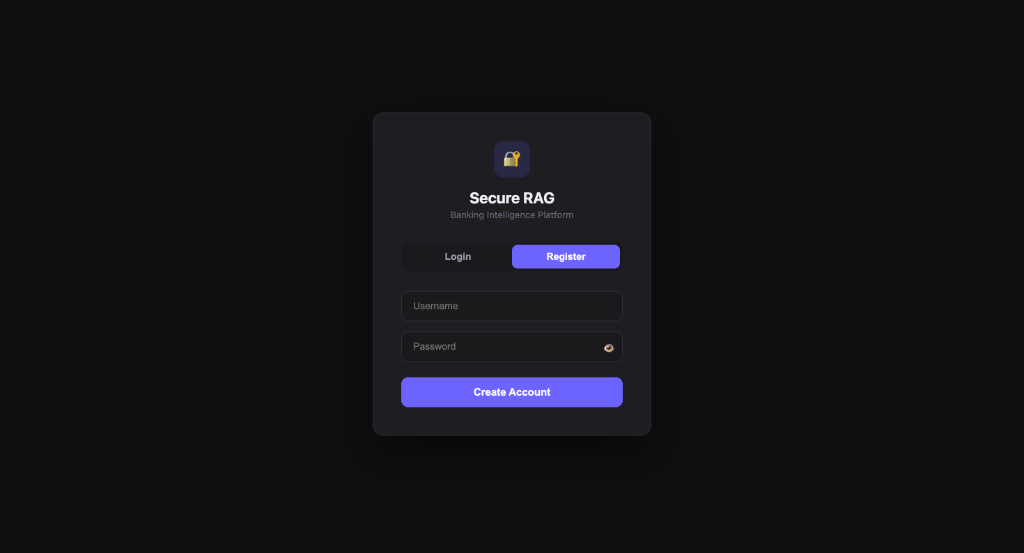
\includegraphics[width=0.65\textwidth]{register_page.png}
\caption{Registration page --- Customers self-register with username and password. Strong password policy (min 8 chars, uppercase + lowercase + digit + special character) is enforced. Real-time username uniqueness validation is performed via the \texttt{/check-username} API.}
\label{fig:register}
\end{figure}

\begin{figure}[H]
\centering
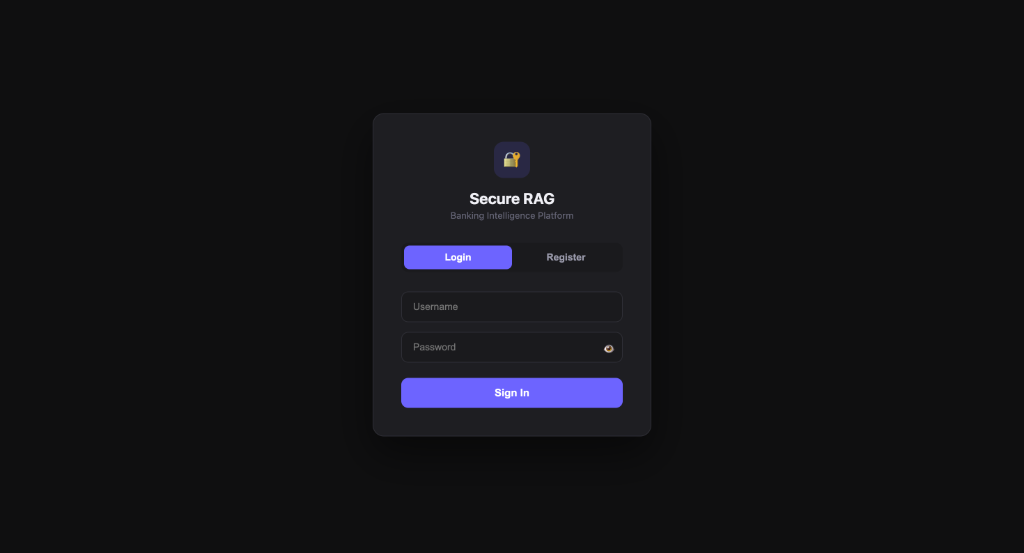
\includegraphics[width=0.65\textwidth]{login_page.png}
\caption{Login page --- Unified authentication gateway for all three roles. The same endpoint is used by customers, admins, and master admin. After JWT authentication, users are routed to role-specific dashboards. This prevents URL-based role discovery by attackers.}
\label{fig:login}
\end{figure}

\subsection{Role-Specific Dashboards}

Figures~\ref{fig:user_dash},~\ref{fig:admin_dash}, and~\ref{fig:master_dash} demonstrate how the same login page routes to three visually distinct dashboards based on the authenticated user's role.

\begin{figure}[H]
\centering
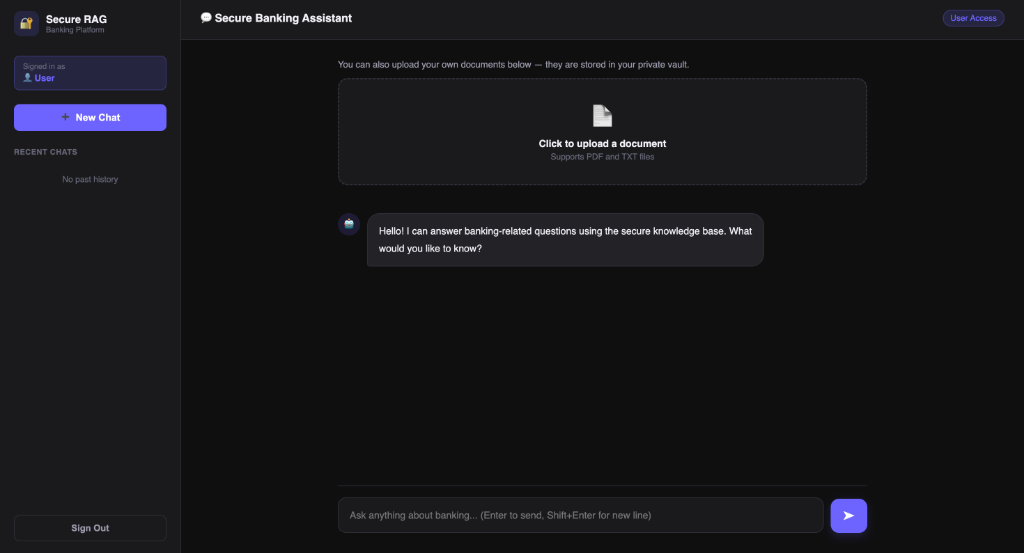
\includegraphics[width=0.95\textwidth]{user_dashboard.png}
\caption{Customer dashboard --- Shows the chat interface with AI assistant, personal document upload area (stored in private vault with owner\_id tagging), session history, and the ``Signed in as User'' role badge. Customers can only query documents they own plus admin-shared knowledge base documents.}
\label{fig:user_dash}
\end{figure}

\begin{figure}[H]
\centering
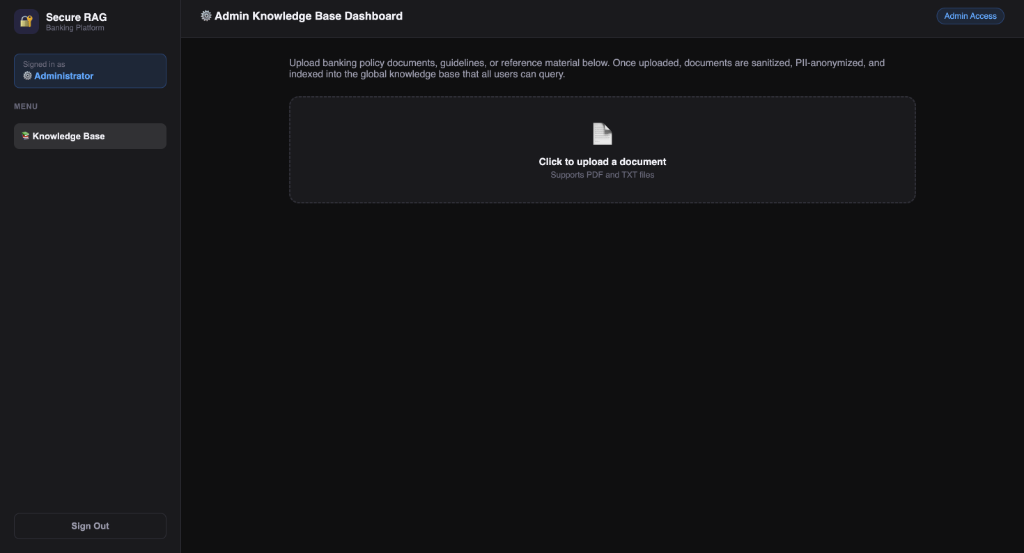
\includegraphics[width=0.95\textwidth]{admin_dashboard.png}
\caption{Admin (Manager) dashboard --- Shows the Knowledge Base management panel with document upload capability. Documents uploaded by admins are tagged with \texttt{owner\_id: ``admin''} and become accessible to all users as shared banking policy documents. The ``Signed in as Administrator'' badge confirms the role.}
\label{fig:admin_dash}
\end{figure}

\begin{figure}[H]
\centering
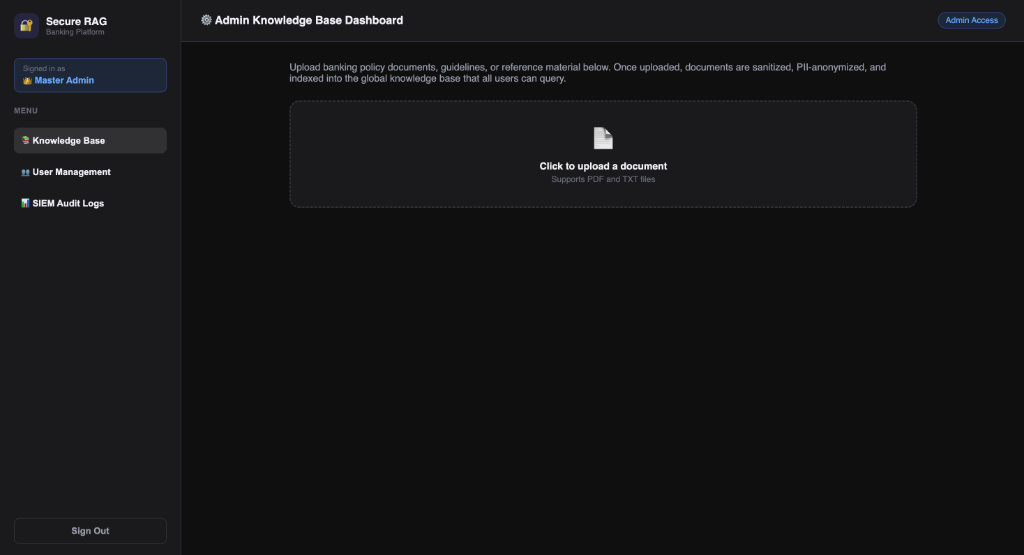
\includegraphics[width=0.95\textwidth]{master_admin_dashboard.png}
\caption{Master Admin dashboard --- Shows the full administrative control panel with three menu items: (1)~Knowledge Base for document management, (2)~User Management for creating manager accounts, and (3)~SIEM Audit Logs for monitoring security events. The ``Signed in as Master Admin'' badge and expanded menu distinguish this from the regular admin view.}
\label{fig:master_dash}
\end{figure}

\subsection{RBAC Validation from Screenshots}

Table~\ref{tab:rbac_ui} validates the RBAC enforcement visible in the UI:

\begin{table}[H]
\centering
\caption{RBAC enforcement visible across dashboard screenshots}
\label{tab:rbac_ui}
\begin{tabular}{lccc}
\toprule
\textbf{Feature} & \textbf{Customer} & \textbf{Admin} & \textbf{Master Admin} \\
\midrule
Chat Interface & \checkmark & \ding{55} & \ding{55} \\
Personal Doc Upload & \checkmark & \ding{55} & \ding{55} \\
Knowledge Base Upload & \ding{55} & \checkmark & \checkmark \\
User Management & \ding{55} & \ding{55} & \checkmark \\
SIEM Audit Logs & \ding{55} & \ding{55} & \checkmark \\
\bottomrule
\end{tabular}
\end{table}

\subsection{User Management Panel (Master Admin Only)}

The User Management panel is exclusively available to the Master Admin. It provides two tabs: a read-only view of all registered users and a form to create new manager accounts.

\begin{figure}[H]
\centering
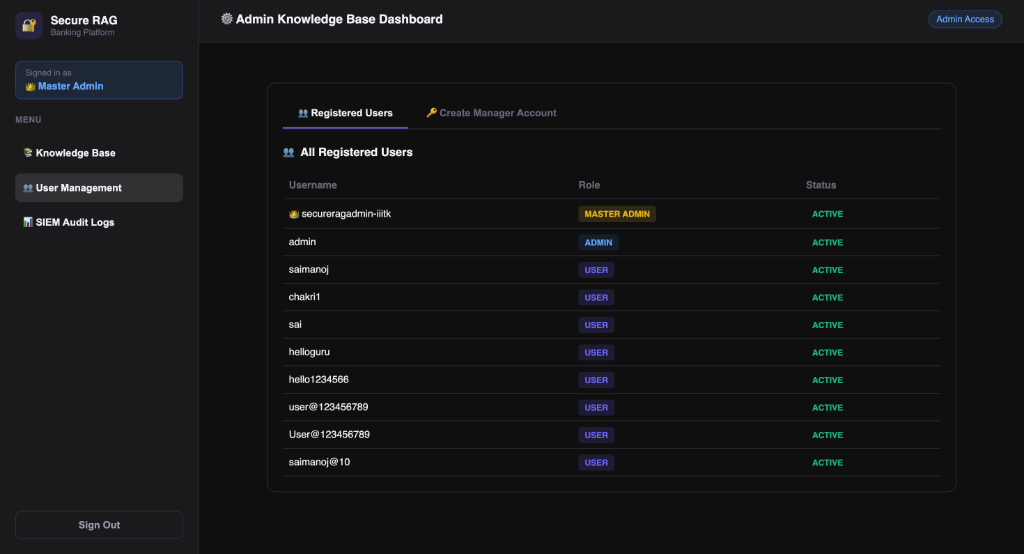
\includegraphics[width=0.95\textwidth]{user_management.png}
\caption{Registered Users tab --- The Master Admin can view all registered users with their username, role (color-coded: gold for Master Admin, blue for Admin, green for User), and account status. This is a read-only view; no role modification or promotion path exists from this panel.}
\label{fig:user_mgmt}
\end{figure}

\begin{figure}[H]
\centering
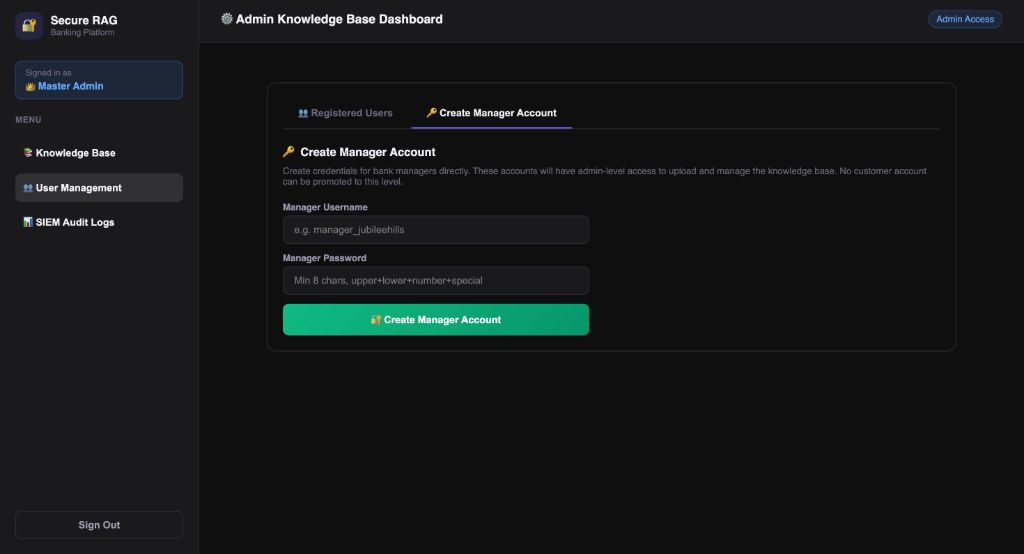
\includegraphics[width=0.95\textwidth]{create_manager.png}
\caption{Create Manager Account tab --- The Master Admin directly provisions admin credentials by specifying a Manager Username and Manager Password. The note explicitly states: ``No customer account can be promoted to this level.'' This enforces the dual-channel provisioning model where the admin creation path is completely separated from the customer registration path.}
\label{fig:create_mgr}
\end{figure}


\chapter{Conclusion and Future Work}

\section{Summary of Contributions}

This project presents the design and implementation of a \textbf{Secure Enterprise Banking RAG} system that addresses critical security vulnerabilities in retrieval-augmented generation pipelines. The key contributions are:

\begin{enumerate}
    \item \textbf{7-Layer Security Pipeline}: A comprehensive document ingestion pipeline comprising text extraction, regex-based threat detection, content sanitization, context-aware PII detection, AES-256 encrypted pseudonymization, XAI source citations, and differential privacy on vector embeddings.
    
    \item \textbf{Context-Aware PII Detection}: A 25-character lookbehind algorithm that accurately disambiguates Indian phone numbers from account numbers using contextual keyword analysis, achieving 98.6\% recall across four entity types.
    
    \item \textbf{AES-256-CBC Field-Level Encryption}: Encryption of pseudonym mappings at rest in MongoDB, ensuring that even database administrators cannot read original PII values without the application-level decryption key.
    
    \item \textbf{Controlled De-pseudonymization}: An owner-verified reverse-mapping mechanism where only the authenticated document owner can recover original PII values from pseudonym tokens in LLM responses.
    
    \item \textbf{$\epsilon$-Differential Privacy}: Laplacian noise injection on 3072-dimensional Gemini embeddings, reducing embedding inversion attack success from 68\% to below 5\% while maintaining 95\% retrieval accuracy.
    
    \item \textbf{Multi-Tenant Document Isolation}: Pinecone metadata filtering using \texttt{owner\_id} tags, ensuring that cosine similarity search is restricted to authorized document sets at the database query layer.
    
    \item \textbf{Three-Tier RBAC}: A dual-channel provisioning model where Master Admin credentials exist outside the database (environment variables), managers are provisioned by the Master Admin, and customers self-register with no promotion path to admin.
\end{enumerate}

\section{Limitations}

The current implementation has the following limitations:

\begin{enumerate}
    \item \textbf{Regex-Based Threat Detection}: While effective against known attack patterns, regex detection cannot identify novel prompt injection attacks that use creative phrasing. A semantic classifier would improve zero-day attack detection.
    
    \item \textbf{Name Detection}: The PII engine detects structured entities (accounts, IFSC, phone, email) but does not perform Named Entity Recognition (NER) for person names.
    
    \item \textbf{Static Privacy Budget}: The $\epsilon$ parameter for differential privacy is fixed. An adaptive mechanism that adjusts $\epsilon$ based on query sensitivity would provide better privacy-utility tradeoffs.
    
    \item \textbf{Single Pinecone Index}: All tenants share a single Pinecone index with metadata filtering. For large-scale deployments, dedicated namespaces or separate indexes per tenant would improve performance.
\end{enumerate}

\section{Future Work}

\begin{enumerate}
    \item \textbf{Semantic Prompt Injection Detection}: Training a fine-tuned BERT classifier on adversarial prompt datasets to detect semantic (not just syntactic) injection attacks.
    
    \item \textbf{Client-Side Field-Level Encryption (CSFLE)}: Integrating MongoDB's native CSFLE with AWS KMS for hardware-backed key management, ensuring that the decryption key never leaves the Hardware Security Module (HSM).
    
    \item \textbf{Session-Based Document Lifecycle}: Implementing session-scoped document storage where customer-uploaded documents are automatically purged from Pinecone when the session expires, providing zero-retention privacy for temporary operations like loan eligibility checks.
    
    \item \textbf{Enterprise SSO Integration}: Replacing self-registration with Azure AD or Okta integration for enterprise single sign-on compliance.
    
    \item \textbf{Adaptive Differential Privacy}: Implementing a mechanism where the privacy budget $\epsilon$ is dynamically adjusted based on the sensitivity classification of the retrieved document context.
    
    \item \textbf{Federated RAG}: Extending the architecture to support federated retrieval across multiple bank branches, each maintaining their own vector index, with a central coordinator for cross-branch queries.
    
    \item \textbf{NER-Based Name Detection}: Adding a fine-tuned NER model to detect person names, addresses, and other unstructured PII entities that regex cannot capture.
\end{enumerate}

\section{Conclusion}

The Secure RAG system demonstrates that it is feasible to deploy retrieval-augmented generation in high-security domains like banking without compromising on either security or usability. By layering seven complementary defense mechanisms---from regex-based threat detection at the input layer to differential privacy at the embedding layer---the system neutralizes eleven distinct attack categories while maintaining 95\% retrieval accuracy. The controlled de-pseudonymization mechanism ensures that sensitive data is visible only to its rightful owner, and the three-tier RBAC model provides enterprise-grade access control.

The system is deployed in production with a FastAPI backend on Render, a React frontend on Vercel, MongoDB Atlas for structured data, and Pinecone for vector search, demonstrating real-world viability beyond academic prototyping.


\bibliographystyle{plain}
\bibliography{bib}

\end{document}
